%Again about two pages long

In this section, we will describe the model of VTSs and the basic constraints imposed by cell biology.

\textbf{The cell as a transport graph:} We consider a cell to be a collection of compartments (nodes) and vesicles (edges), thus defining a transport graph. Every compartment or vesicle has a set of molecular labels, such as SNARE proteins, associated with it.

\textbf{Molecular flows and steady state:} Each edge is associated with a flux of all the molecular types carried by the corresponding vesicle. The total amount of each molecular type on each compartment can therefore increase or decrease. We assume the cell is in a steady state where each compartment’s composition does not vary over short time scales. Therefore, incoming and outgoing fluxes are balanced for each molecular type at each compartment; it is the \textit{stability condition}.

\textbf{Vesicle targeting driven by molecular interactions:} Once a vesicle has budded out of the source, the molecules it carries determine its properties. In particular, for any given pair of a vesicle and a compartment, the set of SNARE proteins that label the former and latter influence whether the vesicle will fuse to that compartment. Biophysically, fusion requires a direct physical interaction between at least one SNARE type on the vesicle and one SNARE type on the compartment. SNAREs fall into two classes (known as Q and R in the cell biology literature) and vesicle fusion requires a pairing of a Q-SNARE with an R-SNARE. The list of molecular pairs that can drive a fusion event is given in a pairing matrix between Q and R SNAREs. Without loss of generality we assume equal numbers of Q and R SNARE types.

\textbf{Molecular regulation:} We assume that for fusion to occur, the pair of SNARE types involved on the vesicle and compartment must both be in an active state. Whether these SNAREs are active or inactive depends on the other molecules found on the vesicle or compartment, respectively. We test many different versions of this kind of molecular regulation. Most generally, the activity state of a given SNARE can be a Boolean function of all the molecular types on a compartment or vesicle. We have also tested \cite{shukla} a particularly simple regulation mechanism in which two SNAREs that can pair to drive fusion inhibit one another; this is the \textit{pairing inhibition}. This is motivated by the idea that pairing must generate an inactive bi-molecular complex.

\textbf{Synthesis:} Given a particular transport graph, a particular labeling of all the compartments and edges, a particular fusion pairing matrix, and a particular regulatory model, we do the following.

\begin{enumerate}
\item We determine which molecules are active on every compartment or vesicle.
\item For every vesicle fusing to a compartment, we determine whether there exists an active pair (one molecule on the vesicle, one on the compartment) which drives that fusion event.
\item For every vesicle-compartment pair where the vesicle does not fuse to the compartment, we verify that there is no pairing of active molecules on the
vesicle and compartment that could drive their fusion.
\item We verify that every molecular type entering a compartment also leaves the compartment, and also that every molecular type entering a set of compartments also leaves that set.
%steady state condition.
\end{enumerate}


%\subsection{Modeling and Symbolic Analysis of VTS: An Overview}
\label{subsec:graphmodel}
%
Since a VTS is a transport graph, it is but natural to formally model
VTS as graphs (as used in computer science) with their nodes denoting
compartments and labeled edges denoting transport vesicles with labels
denoting the set of molecules being transported. The pairing mechanism
can be represented as matching tables over sets of molecules.
% i.e., formally as a boolean function that given requisite labels of nodes and vesicles that returns true if the required regulations are met. 
%
Given such a graph model of VTSs and their properties, such as
stability condition and fusion rules, can be formally defined as
constraints over graphs and uninterpreted Boolean functions.
%
% Note that the formulas define among other things constraints over
% paths between nodes in the graph model of VTS. Similarly, one can
% define fusion rules as constraints over the boolean functions modeling
% the regulations.  
\
% For example, the steady state condition, described informally earlier, can be defined by the formula shown in Listing~1.1.
   
%\begin{itemize}
%\item \srivas{Detailed BIO to Graph problem}
%\end{itemize}


%Given definitions of fusion and budding rules and the steady state conditions, whether a VTS meets maximum connectivity requirement, i.e. the LGC property, can be verified by checking if the formula show in Listing~1.2 is valid.  Here we have defined the property by checking over existence of any fusion/budding rules.  We can eliminate the existential quantifier if we are interested in checking the property for a particular fusion/budding rule.
%
%\subsection{Converting the Graph Problem into Boolean SAT problem}
%\label{subsec:satproblem}
%To convert the graph problem described in sec~\ref{subsec:graphmodeling}, into a boolean SAT problem, we need to define a scheme to represent graphs and boolean functions using a suitable set of propositional variables.  In our earlier work, we modeled the graph problem in C using arrays to model graphs and boolean function.  We then used the CBMC model checker to convert the graph problem into a SAT problem.  One of the challenges we had in our earlier work is dealing with quantifiers.  Note that the connectedness property defined in Listing~1.2 has quantifier alternation.  Even if we were to eliminate the existential quantifier by instantiating the problem for a fixed set of fusion rules, we would have embedded quantifiers in the antecedent of implications.   CBMC supports only a quantifier-free logic n its assertion language.  In our earlier work we used a combination of explicit enumeration at the C-level and clever use f non-determinism to eliminate alternation of quantifiers.  This enumeration was one source of bottleneck for scaling in our earlier work.  In the current work we eliminate this bottleneck by modeling the problem directly as a SAT instance using uninterpreted functions and recursive relations.  The details of te hnew encding will described in subsequent sections.

A VTS is {\em $k$-connected} if every pair of compartments remain
reachable after dropping $k-1$ vesicles.
%
This property of VTSs have been considered informative and
studied by~\cite{shukla}.
%
Here we have build an {\em efficient} tool that studies properties of
VTSs that are not $k$-connected, from some $k$. 

\begin{figure}
\centering
\begin{minipage}{0.50\linewidth}
  \hspace{-4ex}
\begin{tikzpicture}
\matrix [matrix of math nodes,left delimiter=(,right delimiter=),row sep=0.16cm,column sep=0.1cm] (m) {
\times & \times & \times &\times&\times&\times & \times & \times\\
\times & \times & \times&\times&\times&\times& 1 &\times \\
\times & \times & \times&\times&\times&1&\times &\times\\
\times & \times & \times&\times & 1 & \times &\times & \times\\
 \times & \times & \times & \times & \times & \times & \times & \times\\
 \times & \times & \times &\times & \times & \times & \times & \times\\
 \times & \times & \times & \times & \times & \times & \times & \times\\
 \times & \times & \times & \times & \times & \times&\times & \times\\};

\draw[dashed] ($0.5*(m-1-4.north east)+0.5*(m-1-5.north west)$) --
     ($0.5*(m-8-5.south east)+0.5*(m-8-4.south west)$);

\draw[dashed] ($0.5*(m-4-1.south west)+0.5*(m-5-1.north west)$) --
 ($0.5*(m-4-8.south east)+0.5*(m-5-8.north east)$);

\node[above=4pt of m-1-1] (top-1) {$M_1$};
\node[above=4pt of m-1-2] (top-2) {$M_2$};
\node[above=4pt of m-1-3] (top-3) {$M_3$};
\node[above=4pt of m-1-4] (top-4) {$M_4$};
\node[above=4pt of m-1-5] (top-5) {$M_5$};
\node[above=4pt of m-1-6] (top-6) {$M_6$};
\node[above=4pt of m-1-7] (top-7) {$M_7$};
\node[above=4pt of m-1-8] (top-8) {$M_8$};

\node[left=12pt of m-1-1] (left-1) {$M_1$};
\node[left=12pt of m-2-1] (left-2) {$M_2$};
\node[left=12pt of m-3-1] (left-3) {$M_3$};
\node[left=12pt of m-4-1] (left-4) {$M_4$};
\node[left=12pt of m-5-1] (left-5) {$M_5$};
\node[left=12pt of m-6-1] (left-6) {$M_6$};
\node[left=12pt of m-7-1] (left-7) {$M_7$};
\node[left=12pt of m-8-1] (left-8) {$M_8$};


\node[rectangle,above delimiter=\{] (del-top-1) at ($0.5*(top-1.south) +0.5*(top-4.south)$) {\tikz{\path (top-1.south west) rectangle (top-4.north east);}};
\node[above=10pt] at (del-top-1.north) {$Q-Snares$};
\node[rectangle,above delimiter=\{] (del-top-2) at ($0.5*(top-5.south) +0.5*(top-8.south)$) {\tikz{\path (top-4.south west) rectangle (top-6.north east);}};
\node[above=10pt] at (del-top-2.north) {$R-Snares$};

\node[rectangle,left delimiter=\{] (del-left-1) at ($0.5*(left-1.east) +0.5*(left-4.east)$) {\tikz{\path (left-1.north east) rectangle (left-4.south west);}};
\node[left=15pt,rotate=90,xshift=9mm] at (del-left-1.west) {$Q-Snares$};
\node[rectangle,left delimiter=\{] (del-left-2) at ($0.5*(left-5.east) +0.5*(left-8.east)$) {\tikz{\path (left-5.north east) rectangle (left-8.south west);}};
\node[left=15pt,rotate=90,xshift=9mm] at (del-left-2.west) {$R-Snares$};

\begin{pgfonlayer}{myback}

\foreach \element in {m-1-7,m-3-8,m-5-1,m-5-2,m-5-3,m-5-4,m-6-1,m-6-2,m-6-3,m-6-4,m-7-1,m-7-2,m-7-3,m-7-4,m-8-1,m-8-2,m-8-3,m-8-4}{
\highlight[pink]{\element}{\element}
}
\foreach \element in {m-2-7,m-3-6,m-4-5}{
\fhighlight[blue!10]{\element}{\element}
}
\end{pgfonlayer}

\end{tikzpicture}  
\end{minipage}
\begin{minipage}{0.45\linewidth}

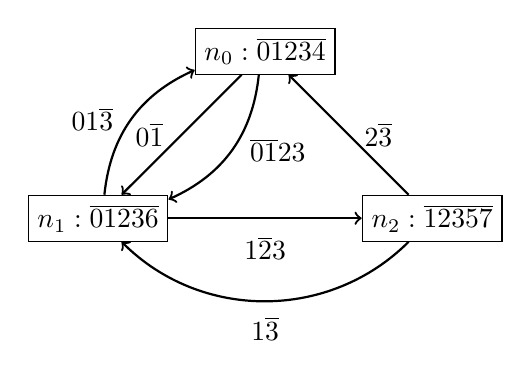
\begin{tikzpicture}[node distance = 30mm]
  \node[draw] (n0) {$n_0:\overline{01234}$};
  \node[draw,below left of=n0] (n1) {$n_1:\overline{01236}$};
  \node[draw,below right of=n0] (n2) {$n_2:\overline{12357}$};

  \draw[->,thick] (n0) -- node[left=1mm]  {$0\overline{1}$} (n1);
  \draw [->,thick] (n0) to [bend right=-30] node[right=1mm]  {$\overline{01}23$} (n1);
  \draw [->,thick] (n1) to [bend right=-30] node[left=1mm]  {$01\overline{3}$} (n0);

  \draw [->,thick] (n1) -- node[below=1mm]  {$1\overline{2}3$} (n2);
  \draw [->,thick] (n2) to [bend right=-45] node[below=2pt]  {$1\overline{3}$} (n1);

  \draw [->,thick] (n2) -- node[right=2pt]  {$2\overline{3}$} (n0);

\end{tikzpicture}
\end{minipage}

\caption{Pairing matrix} \label{fig:M1}
\end{figure}

%%% Local Variables:
%%% mode: latex
%%% TeX-master: "main"
%%% End:


\begin{example}
%
In figure~\ref{fig:M1}, we present a VTS that has 3 compartments and 8 molecules, and a corresponding pairing matrix.
%
Molecules are numbered 0-7.
%
In the VTS, labels are a string of molecule ids, and an overline over an id indicates that the molecule is active.
%
Every molecule on the node is active.
%
The activity of the molecules on an edge are controlled
by presence of the other molecules on the edge.
%
On the right side of the figure, we show the pairing matrix.
%
An entry 1 represents pairing between molecules.
%
$\times$ represents no pairing.
%
Rows corresponds to the labels of edges, and
columns corresponds to the labels of nodes.
%
Every molecule flows on a cycle, ensuring steady state.
%
This is a 3-connected graph.
\end{example}
%--------------------- DO NOT ERASE BELOW THIS LINE --------------------------

%%% Local Variables:
%%% mode: latex
%%% TeX-master: "main"
%%% End:
